\RequirePackage[l2tabu, orthodox]{nag}
\documentclass{ist-report}

% -- Language and text settings
\usepackage{microtype}
\usepackage{xcolor}

% -- Encoding and font
% \usepackage[utf8]{inputenc} -- Use XeLaTeX you dolt
% \usepackage[T1]{fontenc} -- Did I stutter?
% \usepackage{lmodern} -- No.
\usepackage{newpxtext,newpxmath}

% -- Document margins
\usepackage{geometry}
\geometry{verbose, nomarginpar,
    tmargin = 2.5cm,
    bmargin = 2.5cm,
    lmargin = 2.5cm,
    rmargin = 2.5cm}
% \usepackage{showframe}

\usepackage{nimbusmononarrow}

\usepackage{minted}

% -- Bibliography
\usepackage{csquotes}
\usepackage{biblatex}
\addbibresource{main.bib}

% -- Header and footer
\usepackage{footmisc}
\usepackage{fancyhdr}
\fancyhf{}
\pagestyle{fancy}
\fancyhead[L]{}
\fancyhead[C]{}
\fancyhead[R]{Report Example}
\fancyfoot[L]{}
\fancyfoot[C]{}
\fancyfoot[R]{\huge{} \raisebox{-5pt}{
\includegraphics[height = 20pt]{IST_C_CMYK_NEG_CROPPED}} \hspace*{2pt} \vrule{} \hspace*{2pt} \thepage{}}
\renewcommand{\headrulewidth}{0.2pt}
\renewcommand{\footrulewidth}{0pt}

% -- Extra math options
\usepackage{mathtools}
\usepackage{siunitx}

% -- Extra symbols
\usepackage{amssymb}
\usepackage{textcomp}
\usepackage{gensymb}
\usepackage{cancel}

% -- Links and references
\usepackage{hyperref}
\hypersetup{colorlinks,
	linkcolor	= {red!50!black},
	citecolor	= {green!30!black},
	urlcolor	= {blue!80!black}}

% --  Image and float settings
\usepackage{graphicx}
\graphicspath{{graphics/}}
\usepackage{caption}
\usepackage{subcaption}

% -- Graphs and diagrams
\usepackage{tikz}
\usepackage{pgfplots}
\usetikzlibrary{arrows.meta,positioning}
\pgfplotsset{compat=1.5, table/search path = {data}}


\newcommand{\package}[1]{\texttt{#1}}

\begin{document}

\thispagestyle{empty}

\begin{center}
	\vspace{15mm}
	
\includegraphics[width = 0.7\linewidth]{IST_A_CMYK_POS}
	
	{\large Instituto Superior Técnico}\\
	
	\vspace{5mm}
	{\huge\bfseries Report Example}
	
	\vspace{5mm}
	{\LARGE Daniel de Schiffart}
\end{center}

\pagebreak

% Define a lot of characteristics like number commas and exponencials of base 10 and unit representations and stuff
% Also a tree of what happens with which compilers are used, options and whatnot
% Document the TUDelft class file based on the blocks I just defined on the tudelft-report-commented.cls file

{\hypersetup{linkcolor	= black} \tableofcontents}

\pagebreak

\begin{abstract}
	The \LaTeX{} class developed in this project was developed as a template for reports developed for the Instituto Superior Técnico of Universidade de Lisboa, themed around the style the university has developed for its own internal documentation, complemented by using specifications defined by the university itself, all the while taking some creative liberties with the missing definitions.
	
	This document right here is meant as an example to show off most types of content to be typeset, and document the content of the class itself and its effect on the document.
\end{abstract}

\section{Introduction}

This project has the focus on creating a generic \LaTeX{} report example for IST students to base their own reports upon, to streamline much of the typesetting end of things for an IST report so students and other users can focus on writing content instead of spending time getting \LaTeX{} to work. Hopefully it can also work as a first dive for those who want to learn \LaTeX{} a tad more deeply than that. The final goal being having a working example using a custom class file that contains as many definitions as it can with the least possible amount of custom packages, with a couple of simple customisation options, so it can work as a simple template for those who need it. Obviously I'm taking some liberties with how it will end up looking, but hopefully it'll look pretty and professional and presentable and not really as over-the-top as it'd look like if you'd let me loose with Illustrator and a bottle of Jägermeister.

This project also aims to be a learning experience for me. I've only scratched the surface of \LaTeX{} apparently, and looking at examples from other universities made me want to see where I can go before giving up or losing my head. \emph{Obviously} the sane decision in this scenario would be an attempt at creating a class for IST-based reports, much in the vein of what TU Delft did with their \textit{Huisstijl} standardization, which will probably only take up enough time to make me forget to cook every day I mess with it. Hopefully I won't end up copy-pasting \emph{too} much of their work, which I profoundly admire.

A lot of information was acquired from appendix A of \textit{The \LaTeX{} Companion}\cite{latex-companion}, which provided a solid base on how to build a class file based on the needs at hand. I'll keep documenting most other resources as they come up throughout development.

\section{Report Content Samples}

To showcase the class, its effects on multiple \LaTeX{} environments and to give examples on different types of content to use with the class (and with \LaTeX{} in general), this section contains a variety of content to be used within \LaTeX{} and should cover the basis for the content of most reports. Any content not covered here should work fine within this class, as long as there are no conflicting packages, fonts, or other major modifications to the basic \LaTeX{} configuration. Any problems found, report them to me.

\subsection{Basic Math}

This section contains math typesetting as examples to show how it will look like in the final product. This will depend mostly on the font used for math, so the class itself will not have much to change within this department. For the time being, the math font remains imported from the package \package{newpxmath}, which I grew a fondness for. The example from equation \ref{eq:biotsavart} was derived from \textit{The \LaTeX{} Font Catalogue} \cite{fontcatalogue}. It is the integral form of the Biot-Savart law and showcases some details with math font. More math examples to follow.
\begin{gather} \label{eq:biotsavart}
	B(P) = \frac{\mu_0}{4\pi}\int{\frac{\boldsymbol{I} \times \hat{r}'}{r'^2}dl} = \frac{\mu_0}{4\pi} I \int{\frac{d\boldsymbol{l} \times \hat{r}'}{r'^2}}
\end{gather}

An example of arrays and matrices is in equation \ref{eq:sat_error}. The equation in question represents the positioning error $e$ for a group of GPS satellites obtained using differential GPS correction, where $d_{GS}$ represents the distance between satellite $N$ and the differential GPS ground station, and $\rho_{GS}$ the pseudorange obtained in the aforementioned ground station.
\begin{gather} \label{eq:sat_error}
	\left[\begin{matrix}
		e^{(1)} \\
		e^{(2)} \\
		\vdots \\
		e^{(N)} \\
	\end{matrix}\right]
	= \left[\begin{matrix}
		d^{(1)}_{GS} - \rho^{(1)}_{GS} \\
		d^{(2)}_{GS} - \rho^{(2)}_{GS} \\
		\vdots \\
		d^{(N)}_{GS} - \rho^{(N)}_{GS} \\
	\end{matrix}\right]
\end{gather}

\subsection{Floats}

According to the \textit{Wikibooks} \LaTeX{} online textbook \cite{latexwiki},
\begin{quote} \itshape
	Floats are containers for things in a document that cannot be broken over a page. [...] Floats are not part of the normal stream of text, but separate entities, positioned in a part of the page to themselves (top, middle, bottom, left, right, or wherever the designer specifies). They always have a caption describing them and they are always numbered so they can be referred to from elsewhere in the text.
\end{quote}

\subsubsection{Figures}

\subsubsection{Tables}

My apologies for this section, my \LaTeX{} is kinda shoddy when it comes to tables; I've been kinda making it work with basic \texttt{tabular} environments, like the one in table \ref{tab:ex1}.
\begin{table}[ht]
	\centering
	\begin{tabular}{l c c c}
				& Column 1	& Column 2	& Column 3	\\
	\hline
	Line 1		& $0.0$		& $0.1$		& $0.2$		\\
	Line 2		& $0.4$		& $0.5$		& $0.6$		\\
	Line 3		& $0.8$		& $0.9$		& $1.0$
	\end{tabular}
	\caption{Basic table example.}
	\label{tab:ex1}
\end{table}

\subsection{Ti\textit{k}Z}

A basic Ti\textit{k}Z drawing of a tall box can be found in figure \ref{fig:tikz_ex1}.
\begin{figure}[ht]
	\centering
	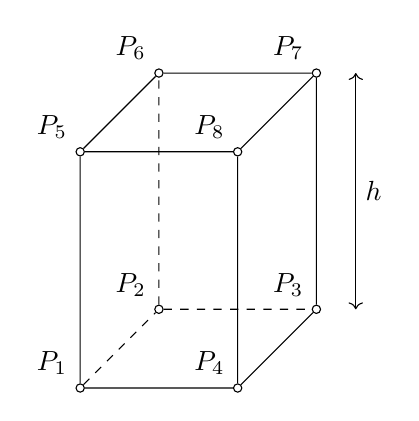
\begin{tikzpicture}[ppoint/.style = {circle,draw,inner sep = 0pt, minimum size = 3pt}]
		\node (p1) at (0,0) [ppoint,label = {135:$P_1$}] {};
		\node (p2) at (1,1) [ppoint,label = {135:$P_2$}] {};
		\node (p3) at (3,1) [ppoint,label = {135:$P_3$}] {};
		\node (p4) at (2,0) [ppoint,label = {135:$P_4$}] {};
		\node (p5) at (0,3) [ppoint,label = {135:$P_5$}] {};
		\node (p6) at (1,4) [ppoint,label = {135:$P_6$}] {};
		\node (p7) at (3,4) [ppoint,label = {135:$P_7$}] {};
		\node (p8) at (2,3) [ppoint,label = {135:$P_8$}] {};
		\draw (p1) -- (p5) -- (p6) -- (p7) -- (p3) -- (p4) -- (p1);
		\draw (p5) -- (p8) -- (p7) (p8) -- (p4);
		\draw [dashed] (p1) -- (p2) -- (p6) (p2) -- (p3);
		\draw [<->] (p3) ++(0.5,0) -- node [auto,swap] {$h$} ++(0,3);
	\end{tikzpicture}
	\caption{Tall box and its corresponding height $h$. Drawing made using Ti\textit{k}Z.}
	\label{fig:tikz_ex1}
\end{figure}

\begin{figure}[ht]
	\centering
	\scalebox{0.8}{
	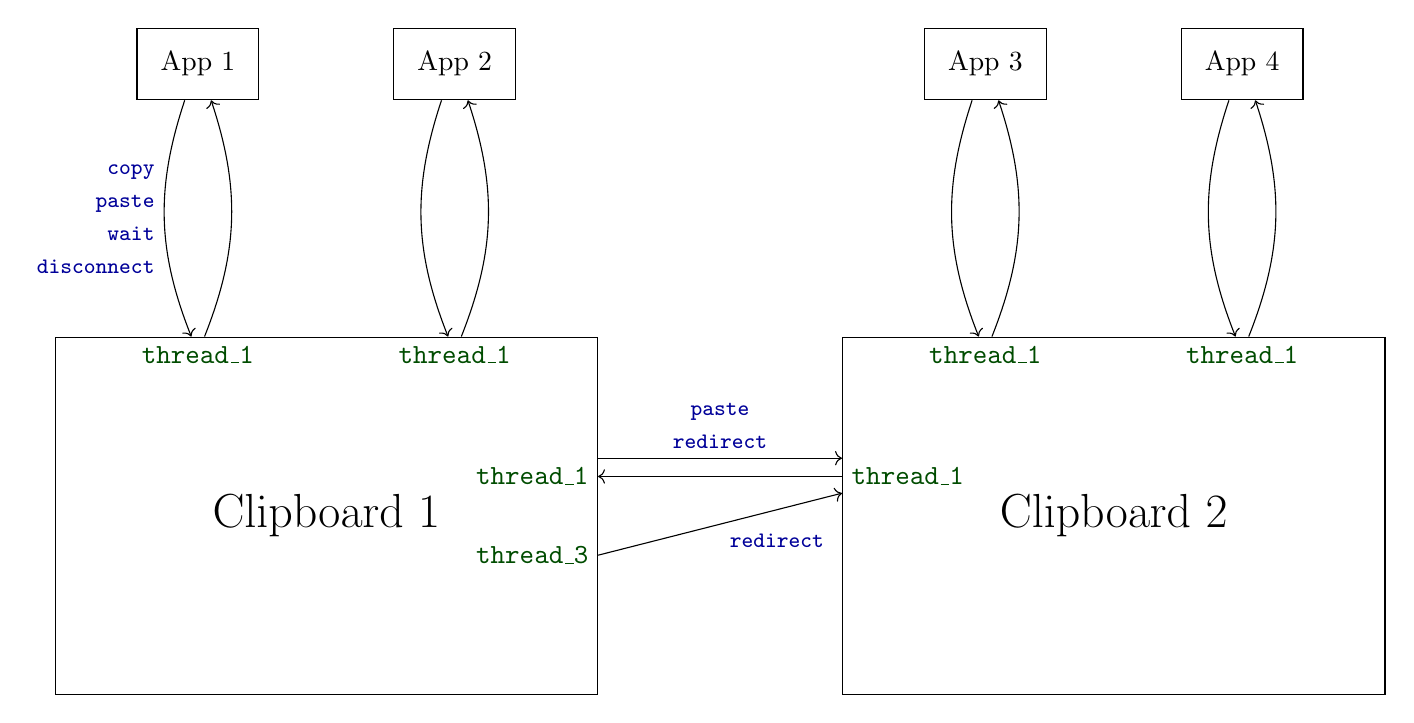
\begin{tikzpicture}[clipboard/.style = {rectangle, draw, inner sep = 2cm},
						app/.style = {rectangle, draw, inner sep = 3mm},
						socketin/.style = {rectangle, color = black!70!green},
						pathstyle/.style = {->},
						pathlabel/.style ={color = black!40!blue}]
		% Start of Clipboard 1
		\node (app1) at (0,0) [app] {App 1};
		\node (app2) [app, right = 1.7cm of app1] {App 2};
		\node (t2app1) [socketin, below = 3cm of app1] {\texttt{thread\_1}};
		\node (t2app2) [socketin, below = 3cm of app2] {\texttt{thread\_1}};
		\draw [pathstyle] (app1) to [bend right = 20] node [auto,swap,align = right, pathlabel] {\footnotesize \ttfamily copy \\ \footnotesize \ttfamily paste \\ \footnotesize \ttfamily wait \\ \footnotesize \ttfamily disconnect} (t2app1);
		\draw [pathstyle] (t2app1) to [bend right = 20] (app1);
		\draw [pathstyle] (app2) to [bend right = 20] (t2app2);
		\draw [pathstyle] (t2app2) to [bend right = 20] (app2);
		\path (t2app1.north) to node (clip1) [auto, swap, clipboard] {\LARGE Clipboard 1} (t2app2.north);
		\path (clip1.north east) to node (clip1in1) [auto, swap, align = right, yshift = 0.5cm, socketin] {\texttt{thread\_1}} node (clip1in3) [auto, swap, align = right, yshift = -0.5cm, socketin] {\texttt{thread\_3}} (clip1.south east);
		% Start of Clipboard 2
		\node (app3) at (10,0) [app] {App 3};
		\node (app4) [app, right = 1.7cm of app3] {App 4};
		\node (t2app3) [socketin, below = 3cm of app3] {\texttt{thread\_1}};
		\node (t2app4) [socketin, below = 3cm of app4] {\texttt{thread\_1}};
		\draw [pathstyle] (app3) to [bend right = 20] (t2app3);
		\draw [pathstyle] (t2app3) to [bend right = 20] (app3);
		\draw [pathstyle] (app4) to [bend right = 20] (t2app4);
		\draw [pathstyle] (t2app4) to [bend right = 20] (app4);
		\path (t2app3.north) to node (clip2) [auto, swap, clipboard] {\LARGE Clipboard 2} (t2app4.north);
		\path (clip2.north west) to node (clip2in1) [auto, align = left, yshift = 0.5cm, socketin] {\texttt{thread\_1}} (clip2.south west);
		% Paths in between
		\draw [pathstyle] (clip1in1.north east) -- node [auto, align = center, pathlabel] {\ttfamily \footnotesize paste \\ \ttfamily \footnotesize redirect} (clip2in1.north west);
		\draw [pathstyle] (clip2in1) -- (clip1in1);
		\draw [pathstyle] (clip1in3.east) -- node [auto, swap, pathlabel] {\ttfamily \footnotesize redirect} (clip2in1);
	\end{tikzpicture}}
	\caption{A slightly longer T\textit{i}kZ example.}
	\label{fig:scheme_main}
\end{figure}

\subsection{Plots}

\subsection{Code Snippets and Extracts}

The objective is to have any code content use the \package{minted} package to typeset code. However, due to the high number of requirements to properly run \package{minted} on a local installation of \TeX{}, this option should only be used with an online editor (\textit{Overleaf} comes as the most prominent example). In any case, for the time being \package{minted} is included in this template, but can be further on replaced with a package like \package{listings}, possibly using a class option. Plans are also down to include a tutorial on how to check and install \package{minted} and get it to work.

Here is a basic excerpt of a basic C \textit{Hello World} program.
\begin{minted}[frame = lines, linenos]{c}
#include <stdio.h>

int main(void)
{
    printf("Hello World!");
    
    return 0;
}
\end{minted}

\section{Class File Documentation}

This section is the most relevant for the class file itself, what it exactly contains, what its options are, and a concise documentation of its development, which will grow as the class file progresses. The class file itself, \texttt{ist-report.cls}, should be in the same directory as the \texttt{main.tex} file.

\subsection{Options}

Currently no options are implemented. The current class carries only default configurations.

\subsection{Packages}

I'm still settling on a way to represent packages, descriptions and links. Until then, they're all listed here in an \texttt{itemize} environment.
\begin{itemize}
	\item \package{mathtools}
	\item \package{babel [portuguese, english]}
\end{itemize}

\subsection{Class Contents}

The class file is based off of the \LaTeX{} basic \package{article} class, edited to fit the Instituto Superior Técnico theme.

\pagebreak

\printbibliography

\end{document}
